\section{Exercise 3}

An application manages the shipment of orders to customers from an inventory. 
The data are organized according to the following conceptual model. 
\begin{figure}[H]
    \centering
    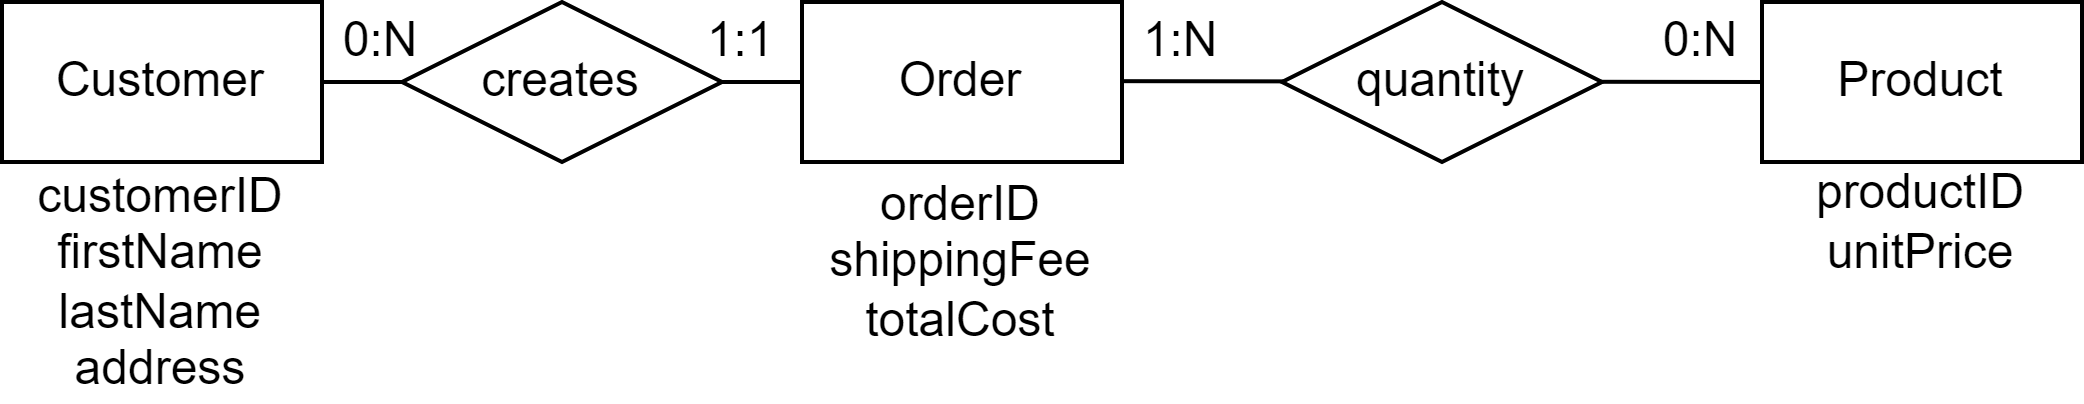
\includegraphics[width=0.75\linewidth]{images/jpa.png}
\end{figure}
The application permits the operator to select a customer, open his/her list of orders, select an order and the list of its products with the ordered quantity associated with each product in the order. 
Customers are in the order of millions, orders per customer are in the order of thousands and products per order are in the order of tens.
Show the JPA entities (with all their attributes) that map the domain objects of the conceptual model, taking into account the above-mentioned access paths of the application and data cardinalities.
When designing the annotations for the relationships, specify the owner side of the relationship, the mapped-by attribute, the fetch policy and the cascading policies you consider more appropriate to support the access required by the web application. 

\paragraph*{Solution}
We start by checking all the relationships in the E-R diagram: 
\begin{itemize}
    \item Orders/orderedBy: from customer to order we have to use the annotations: 
        \begin{lstlisting}[style=Java]
@OneToMany
FetchType.LAZY
        \end{lstlisting}
        From order to customer we have to use these annotations: 
        \begin{lstlisting}[style=Java]
// This annotation can be omitted since it is implicit
@ManyToOne
        \end{lstlisting}
        The owner of the relation is order. 
    \item Contains/containedIn: from order to product we have to use the annotations: 
        \begin{lstlisting}[style=Java]
FetchType.EAGER
        \end{lstlisting}
        From product to order we have to use these annotations: 
        \begin{lstlisting}[style=Java]
// This annotation can be omitted since it is implicit
@ManyToMany
        \end{lstlisting}
        The owner of the relation is product. 
\end{itemize}
We can now define the three entity mappings. 
The entity customer is defined as:  
\begin{lstlisting}[style=Java]
@Entity
public class Customer implements Serializable {

    @Id @GeneratedValue(strategy = GenerationType.AUTO)
    private int customerId;
    private String firstName;
    private String lastName;
    private String address;

    @OneToMany(mappedBy="customer", fetch = FetchType.LAZY)
    private List<Order> orders;
    . . .
}
\end{lstlisting}
The entity product is defined as:  
\begin{lstlisting}[style=Java]
@Entity
public class Product implements Serializable {

    @Id @GeneratedValue(strategy = GenerationType.AUTO)
    private int productId;
    private int unitPrice;

    @ManyToMany
    @JoinTable(name = "product_order",
               joinColumns = @JoinColumn(name = "productId"),
               inverseJoinColumns = @JoinColumn(name ="orderId"))
    private List<Order> orders; 
    . . .
}
\end{lstlisting}
The entity order is defined as:  
\begin{lstlisting}[style=Java]
@Entity
public class Order implements Serializable {

    @Id @GeneratedValue(strategy = GenerationType.AUTO)
    private int orderId;
    private int shippingFee;
    private int totalCost;

    @ManyToOne
    @JoinColumn(name="customer") 
    private Customer customer;

    @ElementCollection(fetch = FetchType.EAGER)
    @CollectionTable(name = "product_order",
    joinColumns = @JoinColumn(name = "orderId"))

    @MapKeyJoinColumn(name = "productId") 
    @Column(name = "quantity")
    private Map<Product, Integer> products;
    . . .
}
\end{lstlisting}